\documentclass[12pt, a4paper] {article}

\usepackage[utf8]{inputenc}
\usepackage[russian]{babel}
\usepackage{amsmath,amssymb,mathrsfs, amsfonts, amsthm}
\usepackage{ upgreek }
 %\usepackage[dvips]{graphicx}

\usepackage{tikz}
%\usepackage{verbatim}
%\usetikzlibrary{calc}

\newcommand{\Z}{\mathbb{Z}}
\newcommand{\R}{\mathbb{R}}
\newcommand{\N}{\mathbb{N}}
\DeclareMathOperator{\tr}{tr}
\DeclareMathOperator{\diam}{diam}
\DeclareMathOperator{\Vol}{Vol}
\DeclareMathOperator{\interior}{int}


 \newtheorem{theorem}{Теорема}[section]
 \newtheorem{theor}[theorem]{Теорема}
 \newtheorem{lemma}[theorem]{Лемма}
\newtheorem{conseq}[theorem]{Следствие}
\newtheorem{prop}[theorem]{Предложение}
\newtheorem{hyp}[theorem]{Гипотеза}
\newtheorem{condition}[theorem]{Условия}

\newtheorem{example}[theorem]{Пример}
\theoremstyle{remark}
 \newtheorem{remark}[theorem]{Замечание}
\theoremstyle{definition}
 \newtheorem{defin}{Определение}


 \def\proof{\noindent{\it Доказательство.~~}}

%\usepackage{tikz}
%\usepackage{verbatim}
%\usetikzlibrary{calc}

\def\l{\left}
\def\r{\right}

\begin{document}

\newcommand{\address}{{
\bigskip
\footnotesize
\textsc{Московский государственный университет им. М.В. Ломоносова,
механико-математический факультет, Москва}\par\nopagebreak
}}


\title{Приближённое решение дифференциального уравнения}

\author{Отчёт студента 410 группы Михайлина Дмитрия Александровича} %\\ 

%\udk{517.518.36}

\maketitle

\section{Постановка задачи}
Решить дифференциальное уравнение:
\begin{gather}
	\label{1} \frac{d^2x}{dt^2} + (1 + \alpha x^2)x = \cos(t), 	 \alpha = 0.2, -0.2
\end{gather}
Сами зададим начальные условия.
Перепишем $\ref{1}$ в виде системы двух дифференциальных уравнений:
\begin{gather}
 \ref{1} \Leftrightarrow 
 \begin{cases}
 \frac{dx}{dt} = y \\
 \frac{dy}{dt} = \cos(t) - (1 + \alpha x^2)x
 \end{cases}
\end{gather}
Получается мы свели дифференциальное уравнение второго порядка к системе дифференциальных уравнений.
Будем решать эту систему при помощи метода Дормана-Принса 7 порядка.

Введём обозначения:

Пусть s - целое положительное число, называемое числом стадий и $a_{21}, \dots a_{s,s-1}, b_{1}, \dots b_{s}, c_{2} \dots c_{s}$ - вещественные коэффициенты. Тогда метод
\begin{gather}
k_1 = f (x_0, y_0) \nonumber\\
k_2 = f (x_0 + c_2h, y_0 + h a_{2,1} k_1) \nonumber \\
k_3 = f (x_0 + c_3h, y_0 + h (a_{3,1} k_1 + a_{32} k_2) \nonumber\\
\dots \nonumber\\
k_s = f (x_0 + c_s h, y_0 + h(a_{s,1} k_1 + \dots + a_{s,s-1}k_{s-1} ))\nonumber \\
y_1 = y_0 + h (b_1k_1 + \dots b_s k_s))
\end{gather} - будет $s$-стадийным явным методом Рунге-Кутта, решения задачи:
\begin{gather}
\begin{cases}
y' = f(x, y) \\
y(x_0) = y_0
\end{cases}
\end{gather}
%Обычно коэффициенты удовлетворяют:
%$c_i = \sum_i a_{ij}$
\begin{defin}
Метод Рунге-Кутты имеет порядок $p$, если:
 $$ || y(x_0 + h) - y_1 || \le Kh^{p+1},$$
 т.е члены для точного решения $y(x_0 + h)$ и для $y_i$ совпадают до члена $h^p$ включительно.
\end{defin}
Приведем таблицы Бутчера из книги Хайрер Э., Нерсетт С., Ваннер Г. "Решение обыкновенных дифференциальных уравнений. Нежесткие задачи", которыми будем пользоватся: \\
Таблица Бутчера метода Рунге-Кутта 6 порядка.\\
\begin{figure}[h!]
\centering
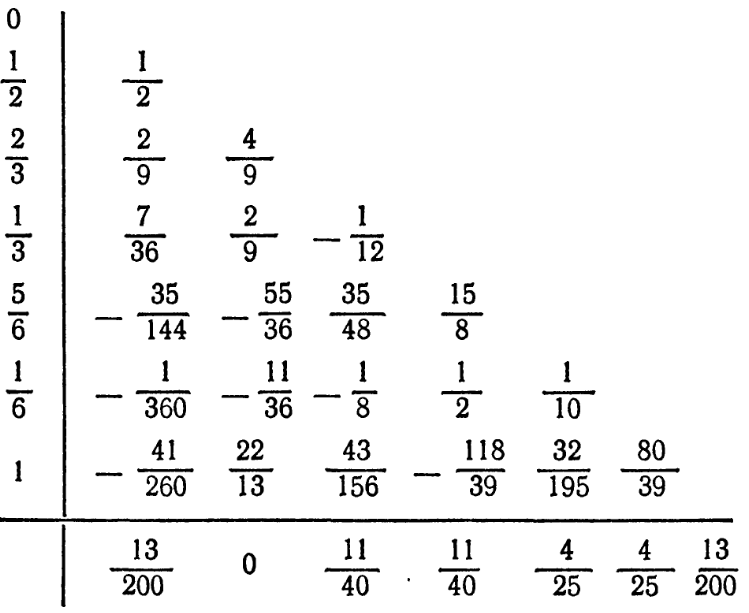
\includegraphics[width=0.5\linewidth]{butcher6.png} 
\end{figure}
\\
$c_i$ находятся в первом столбце, $a_{i,j}$ - располагаются как матрица во всех остальных строках и столбцах, последний столбец соответствует  $b_s.$

Согласно теореме на стр. 202, используя данную таблицу, мы можем построить приближение 6 порядка.\\
Так же приведем таблицу Бутчера для метода Дормана-Принса 8(7) порядка.\\
\\\begin{figure}[h!]
\centering
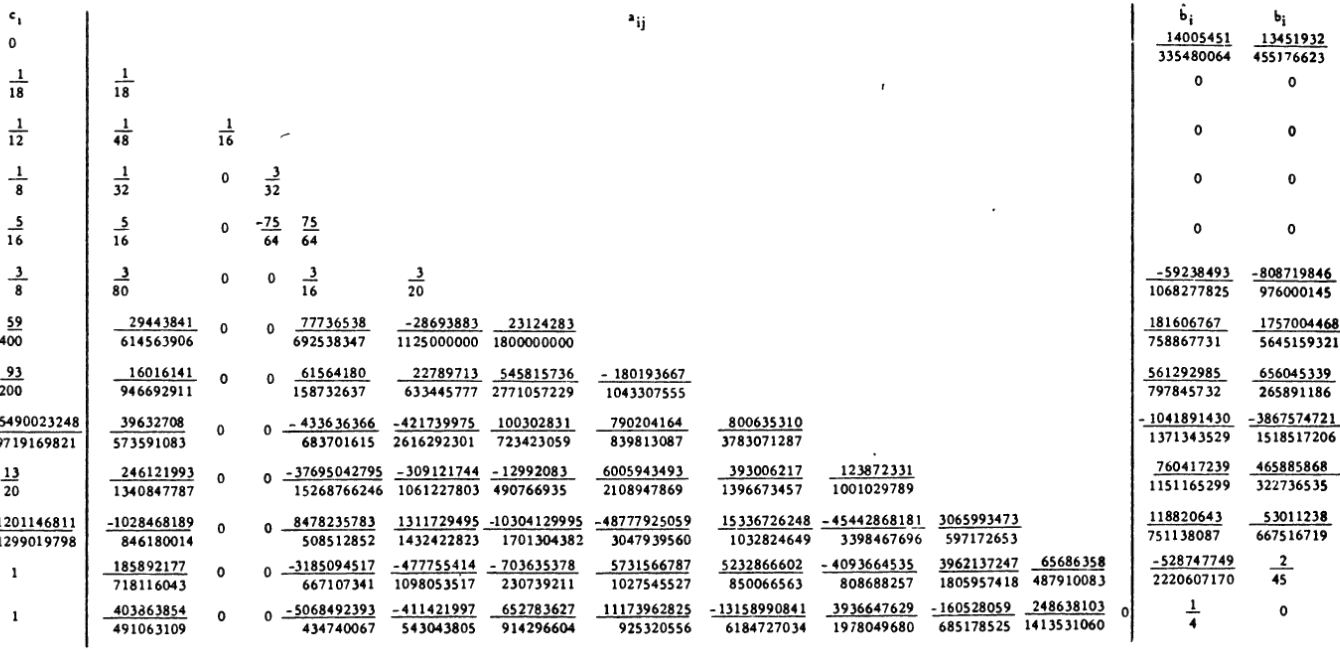
\includegraphics[width=1\linewidth]{dp78.png} 
\end{figure}
\\
\\
\\ \\ \\ \\ \\ \\ \\ \\ \\ \\ \\ \\ \\ 
\section{Переменный шаг:}

\textbf{Правило Рунге:}\\
Пусть заданы точка $(x)$ и приближение $y^{(1)} (x)$ к $y(x)$ -- из обычной задачи Коши, вычисленное через таблицу Бутчера (методом Рунге-Кутта) с шагом $2h.$
Часто в ходе расчётов целесообразно изменять шаг интегрирования, контролируя величину погрешности метода на шаге. При практической оценке этой величины можно, например, рассуждать следующим образом. Главный член погрешности на шаге интегрирования есть;
$$\frac{\varphi^{(s+1)} (0) h^{s+1}}{(s+1)!}$$
Посчитаем приближение вычисленное в точке $(x+h)$: $y^{(2)}(x)$ через таблицу Бутчера (методом Рунге-Кутта) с шагом h, за две итерации.

В результате двух шагов имеем:
$$y^{(1)} - y(x + 2h) \approx \frac{\varphi^{s+1}(0) (2h)^{s+1}}{(s+1)!}$$
Из этих соотношений получаем представление главного члена погрешности на шаге:
$$y^{(1)} - y(x + 2h) \approx \frac{y^{(2)} - y^{(1)}}{2^s - 1} \Rightarrow y(x + 2h) \approx y^{(1)} + \frac{y^{(1)} - y^{(2)}}{2^s - 1}$$\\
Далее посчитаем ошибку. $ err = \frac{||y^{(1)} - y^{(2)}||}{2^s - 1}$, где s - порядок метода. В качестве нормы возьмем $ ||x|| = max|x_i|$.Если ошибка меньше наперед заданного $tol$ то мы принимаем эти два шага. $h$ длину шага пересчитываем по следующей формуле: $h_{new} =h_{old}*min(facmin, max(facmax, fac*(\frac{err}{tol})^\frac{1}{7}))$. facmax, facmin, fac - это константы, которые выбираются для того, чтобы h не убывала слишком быстро и не возрастала слишком быстро. Это повышает надежность программы. Такой выбор шага называется \textbf{Правилом Рунге}.\\
\textbf{Выбор шага в алгоритме Дормана-Принса:}\\
Cначала вычисляем $y^{(1)}$ - приближенное значение в точке $x_0 + h$ методом Рунге-Кутта 7 порядка. Потом вычисляем $y^{(2)}$ приближенное значение в точке $x_0 + h$ уже методом 8 порядка. Рассматриваем ошибку как $err = || y^{(1)} - y^{(2)}||$. Если $err < tol$ - то шаг принимается. Новый шаг h пересчитывается по формуле $h_{new} = h_{old}*min(facmin, max(facmax, fac*(\frac{err}{tol})^\frac{1}{7}))$.

\section{Гармонический осциллятор}
Рассмотрим работу алгоритмов RK-6, RK-7, RK-8 с выбором шага по правилу Рунге и алгоритма DP-8(7) на гармоническом осцилляторе.\\
\begin{gather}
	x'' + \omega^2x = 0
\end{gather}
Перепишем это дифференциальное уравнение в следующем виде:
\begin{gather}
\begin{cases}
	x' = y\\
	y' = -\omega^2x
\end{cases}
\end{gather}
В следующих таблицах приводятся результаты работы алгоритмов \\на $[0, 10\pi], [0, 100\pi], [0, 1000\pi], [0, 10000\pi]$.
\begin{table}
\caption{\label{tab:canonsummary}$[0, 10\pi]$.}
\begin{center}
\begin{tabular}{|c|c|c|c|c|с|c|}
\hline
Алг.: & Погр в $10\pi$ & Макс. погр. & Мин. шаг & Макс. шаг & Сред. шаг & Кол-во шагов \\
\hline
RK-6 & 6.16094e-08 & 6.16094e-08 & 0.0294031 & 0.124017 & 0.118662 &  265 \\
\hline
RK-7 & 1.01278e-08 & 1.53735e-08 &  0.1 & 0.429062 & 0.387965 & 81 \\
\hline
RK-8 & 4.3534e-09 & 6.37778e-09 & 0.0416447 & 0.593831 & 0.499327 & 63\\
\hline
DP-7 & 4.13717e-10 & 6.5382e-10 & 0.1 & 0.43188 & 0.402768 & 78 \\
\hline
\end{tabular}
\end{center}
\end{table} 

\begin{table}
\caption{\label{tab:canonsummary}$[0, 100\pi]$.}
\begin{center}
\begin{tabular}{|c|c|c|c|c|с|c|}
\hline
Алг.: & Погр в $100\pi$ & Макс. погр. & Мин. шаг & Макс. шаг & Сред. шаг & Кол-во шагов \\
\hline
RK-6 &  6.19492e-07 &  6.19492e-07  & 0.1 & 0.124017 & 0.119879 &  2621 \\
\hline
RK-7 & 1.00721e-07 & 1.63357e-07 &  0.0392214 & 0.429062 & 0.409646 & 767 \\
\hline
RK-8 & 1.61544e-08 & 6.87135e-08 & 0.1 & 0.593831 & 0.566994 & 555\\
\hline
DP-7 & 2.65332e-09 & 4.47656e-09 & 0.1 & 0.433579 & 0.433579 & 753 \\
\hline
\end{tabular}
\end{center}
\end{table} 

\begin{table}
\caption{\label{tab:canonsummary}$[0, 1000\pi]$.}
\begin{center}
\begin{tabular}{|c|c|c|c|c|с|c|}
\hline
Алг.: & Погр в $1000\pi$ & Макс. погр. & Мин. шаг & Макс. шаг & Сред. шаг & Кол-во шагов \\
\hline
RK-6 &  6.19848e-06 &  6.20021e-06 & 0.1 & 0.124017 & 0.119933 &  26195 \\
\hline
RK-7 & 7.86173e-07 & 1.63662e-06 &  0.1 & 0.429062 & 0.413014 & 7607 \\
\hline
RK-8 & 2.67748e-07 & 6.99391e-07 & 0.1 & 0.593831 & 0.572827 & 5485\\
\hline
DP-7 & 2.67163e-08 & 4.30018e-08 & 0.1 & 0.433578 & 0.418991 & 7498 \\
\hline
\end{tabular}
\end{center}
\end{table} 

\begin{table}
\caption{\label{tab:canonsummary}$[0, 10000\pi]$.}
\begin{center}
\begin{tabular}{|c|c|c|c|c|с|c|}
\hline
Алг.: & Погр в $10000\pi$ & Макс. погр. & Мин. шаг & Макс. шаг & Сред. шаг & Кол-во шагов \\
\hline
RK-6 &  6.20938e-05 &  6.21198e-05 & 0.1 & 0.124017 & 0.119938 &  261935 \\
\hline
RK-7 & 6.45327e-06 & 1.64321e-05 &  0.1 & 0.429062 & 0.413257 & 76021 \\
\hline
RK-8 & 3.48813e-06 & 7.04343e-06 & 0.1 & 0.593831 & 0.573486 & 54781\\
\hline
DP-7 & 2.65863e-07 & 4.29382e-07 & 0.1 & 0.433595 & 0.419142 & 74953 \\
\hline
\end{tabular}
\end{center}
\end{table} 

\\
\textbf{Графики гармонического осциллятора $[0, 10\pi]$}\\
\\
\begin{figure}[h!]
RK-6 $[0, 10\pi]$ \\
\centering
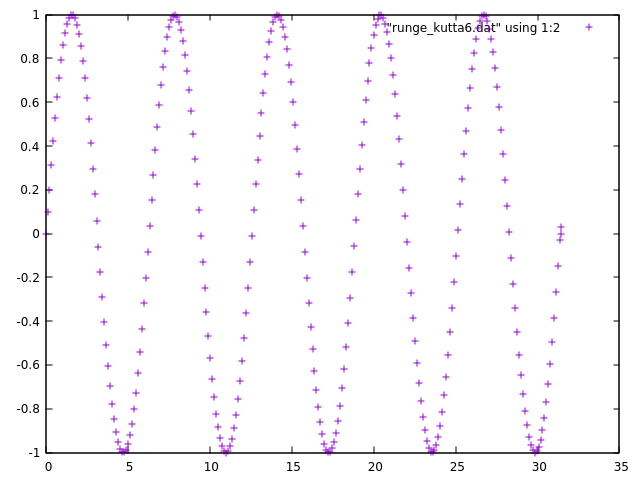
\includegraphics[width=0.5\linewidth]{rk-6.png} 
\end{figure}
\newpage
\begin{figure}[h!]
RK-7 $[0, 10\pi]$ \\
\centering
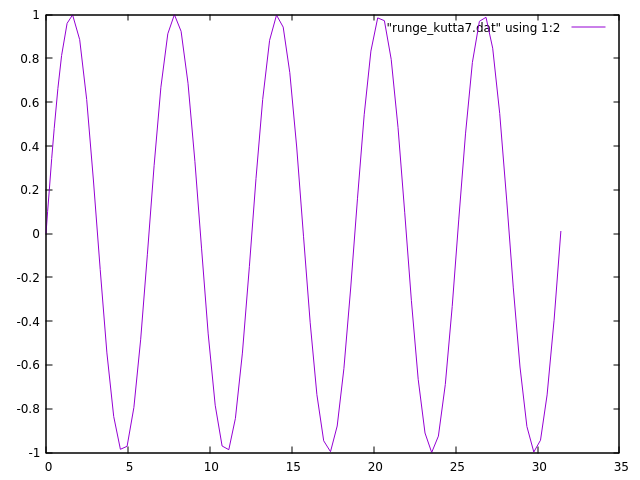
\includegraphics[width=0.5\linewidth]{rk-7.png} 
\end{figure}
\begin{figure}[h!]
RK-8 $[0, 10\pi]$ \\
\centering
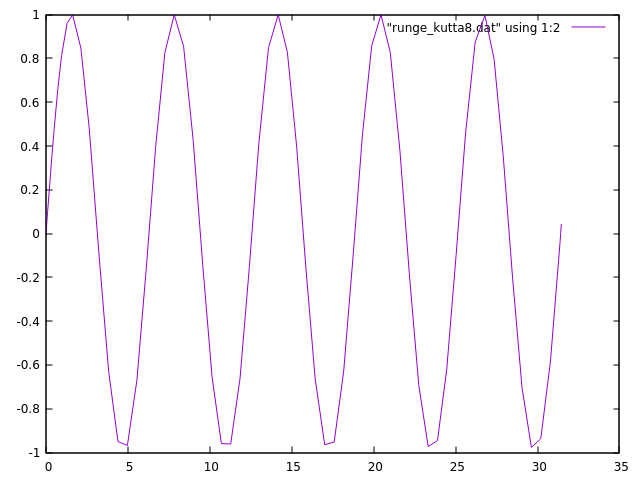
\includegraphics[width=0.5\linewidth]{rk-8.png} 
\end{figure}
\begin{figure}[h!]
DP-7 $[0, 10\pi]$ \\
\centering
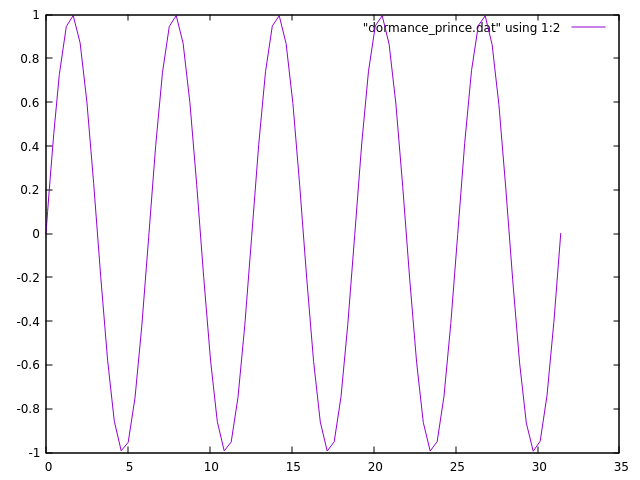
\includegraphics[width=0.5\linewidth]{dp-7.png} 
\end{figure}
\newpage
Таким образом, DP-7 ,несмотря на меньший порядок точности основного метода чем у RK-8 в итоге показывает большую точность, из-за лучшего выбора шага. Если сравнить DP-7 и RK-7, то DP-7 при меньшем количестве узлов показывает гораздо лучшую точность. \textbf{Далее везде используем DP-7}
.\\

\section{Поиск периода}
Сначала ищем такое минимальное t, что $y(x(t)) = 0$. Пусть это будет $t_0$. Далее идем по фазовому портрету и ищем место, где $y(x(t))$ меняет знак. Ищем корень методом хорд. Хотим найти такое T, что:
\begin{gather}
\begin{cases}
\notag x(t_0) = x(t_0 + T), \\
\notag y(t_0) = y(t_0 + T)
\end{cases}
\end{gather}
Такое минимальное T и принимаем за ответ.
\\
\textbf{Период осциллятора}
\begin{gather}
\begin{cases}
\notag x' = y \\
\notag y' = -x \\
\notag x(0) = 0 \\
\notag y(0) = 1
\end{cases}
\end{gather}
\begin{figure}[h!]
 Osc \\
\centering
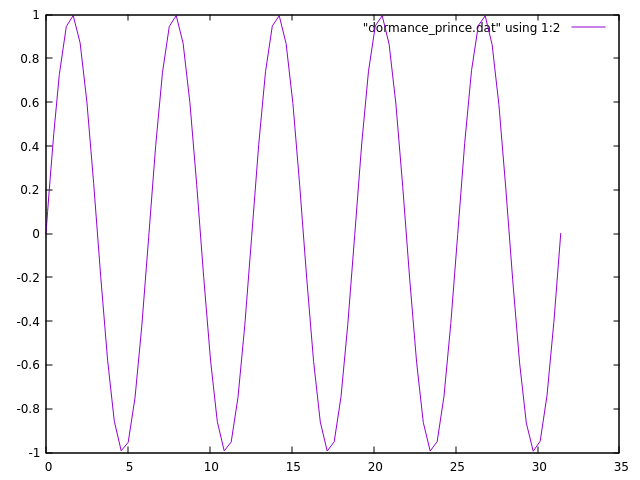
\includegraphics[width=0.5\linewidth]{osc2pi} 
\end{figure}
$T \approx 6.28319 \approx 2\pi$\\

\begin{gather}
\begin{cases}
\notag x' = y \\
\notag y' = -4x \\
\notag x(0) = 0 \\
\notag y(0) = 2
\end{cases}
\end{gather}
\begin{figure}[h!]
Osc \\
\centering
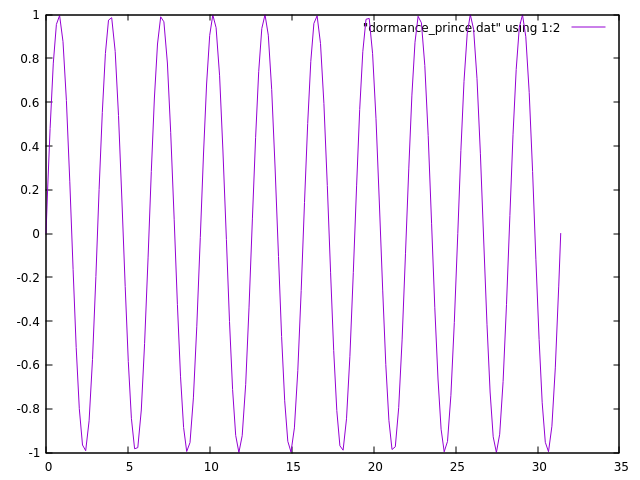
\includegraphics[width=0.5\linewidth]{oscpi.png} 
\end{figure}
\newpage
$T \approx 3.14159 \approx \pi$\\
\section{Графики задачи и период}
\begin{gather}
\begin{cases}
\notag x' = y \\
\notag y' = -(1 + 0.2x^2)x + cos(t) \\
\notag x(0) = 0 \\
\notag y(0) = 1
\end{cases}
\newpage
\end{gather}
\begin{figure}[h!]
$[0, 10]$ \\
\centering
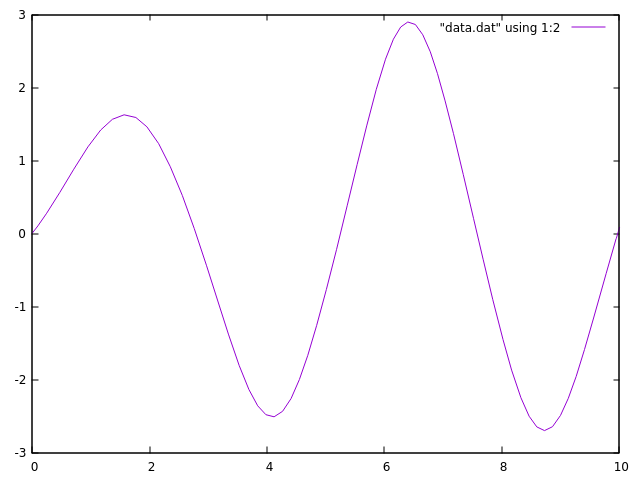
\includegraphics[width=1\linewidth]{solve_plus.png} 
\end{figure}

\newpage
\begin{figure}[h!]
$[0, 100]$ \\
\centering
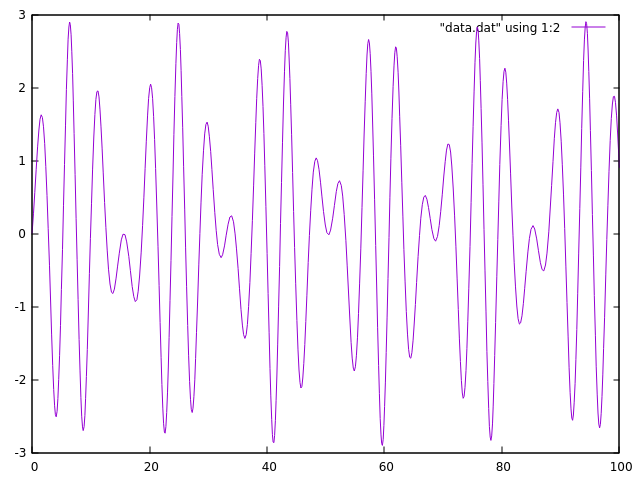
\includegraphics[width=1\linewidth]{sovle_plus_100.png} 
\flushleft
\end{figure}

\newpage
\begin{figure}[h!]
$[0, 250]$ \\
\centering
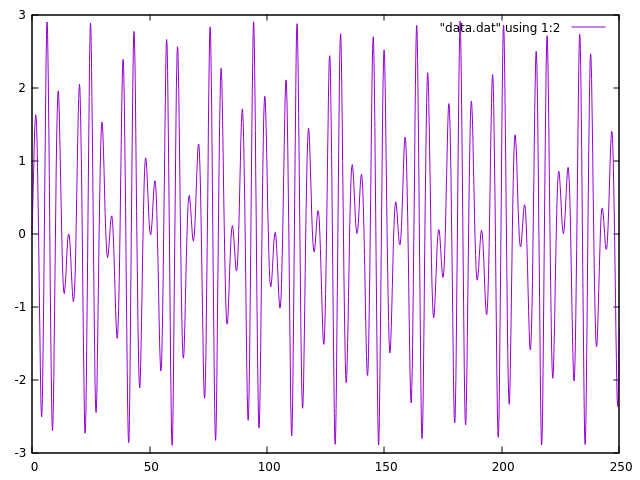
\includegraphics[width=1\linewidth]{solve_plus_250.png} 
\end{figure}
$T \approx 4677.78$
\newpage
\begin{gather}
\begin{cases}
\notag x' = y \\
\notag y' = -(1 - 0.2x^2)x + cos(t) \\
\notag x(0) = 0 \\
\notag y(0) = 1
\end{cases}
\end{gather}
Решение не периодическое.
\begin{figure}[h!]
$[0, 3.8]$ \\
\centering
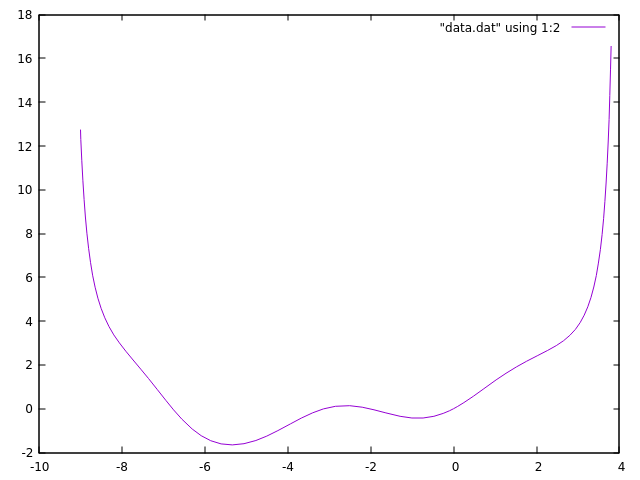
\includegraphics[width=1\linewidth]{min_3.png} 
\end{figure}
\newpage
\begin{gather}
\begin{cases}
\notag x' = y \\
\notag y' = -(1 - 0.2x^2)x + cos(t) \\
\notag x(0) = 0 \\
\notag y(0) = -1
\end{cases}
\end{gather}
Решение не периодическое.
\begin{figure}[h!]
$[0, 9]$ \\
\centering
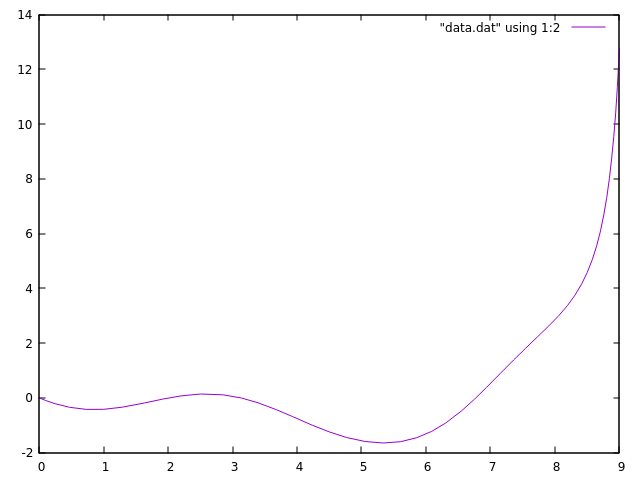
\includegraphics[width=1\linewidth]{min_0_9.png} 
\end{figure}


\end{document}